\documentclass[french]{article}
\usepackage{makecell}

\usepackage[utf8]{inputenc} % encode en UTF8

\usepackage[T1]{fontenc}





\usepackage[top=2cm, bottom=2cm, left=3cm, right=3cm]{geometry}
\usepackage{graphicx}
\usepackage{caption}
\usepackage{subcaption}
\usepackage{float}
\graphicspath{ {./photo/} }

%Belles fraction de fration \cfrac
\usepackage{amsmath}

\usepackage{tikz}
\usepackage{circuitikz}
\renewcommand{\contentsname}{Table des matières}
\renewcommand{\listfigurename}{Table des figures}
\renewcommand{\listtablename}{Liste des tableaux}


\parindent=0cm 

\usepackage{listings}             % Include the listings-package

\lstset{language=Matlab}          % Set your language (you can change the language for each code-block optionally)



%\lstdefinestyle{CStyle}{
%	backgroundcolor=\color{backgroundColour},
%	commentstyle=\color{mGreen},
%	keywordstyle=\color{magenta},
%	numberstyle=\tiny\color{mGray},
%	stringstyle=\color{mPurple},
%	basicstyle=\footnotesize,
%	breakatwhitespace=false,
%	breaklines=true,
%	captionpos=b,
%	keepspaces=true,
%	numbers=left,
%	numbersep=5pt,
%	showspaces=false,
%	showstringspaces=false,
%	showtabs=false,
%	tabsize=2,
%	language=C
%}




\newcommand{\HRule}{\rule{\linewidth}{0.5mm}} % Epaisseur des lignes horizontales

\pagestyle{empty}
\newcommand{\myTitle[1]}{
\begin{minipage}{.47\textwidth}
\centering
\begin{flushleft}

\includegraphics[width=0.75\textwidth]{./photo/nantes_universite_logo.png}
\end{flushleft}
\end{minipage}
\begin{minipage}{.47\textwidth}
\centering
\begin{flushright}
\hspace*{1cm} 
\includegraphics[width=0.85\textwidth]{./photo/logo_polytech_nantes}
\end{flushright}
\end{minipage}~\\[1.5cm]

\begin{center}
\vspace*{\stretch{0.3}}
\end{center}

\begin{center}
  \Large
  \vspace*{\stretch{1}}
  \HRule \\[0.2cm]
  \begin{center}
    \huge
    \textbf{#1}\\ %Titre
  \end{center}
  %\textbf{\\ Projet Transversal}\\ %matière
  \HRule \\[1.5cm]
  
%  \vspace*{\stretch{5}}
%  
%  \small
%  \noindent Rédigé par \\
%  \vspace*{\stretch{0.2}}
%  \large
%  \noindent \Redac\\
%  \vspace*{\stretch{0.5}}
 
\end{center}

\vspace*{\stretch{2}}

\begin{center}\large
	\textsc{École Polytech de Nantes}\\
	\textsc{Département Électronique et Technologie du Numérique}
\end{center}

\vspace*{\stretch{5}}

\begin{center}
	\begin{minipage}{0.4\textwidth}
		\begin{flushleft} \large
        	\noindent Rédigé par\\ %\Redac
			Mathis BRIARD \\
			Victor DUFRENE
		\end{flushleft}
	\end{minipage}
	\begin{minipage}{0.4\textwidth}
		\begin{flushright}\large
			Professeur encadrant : \\Olivier PASQUIER
		\end{flushright}
	\end{minipage}
\end{center}
}


\begin{document}
	\myTitle[Rapport d'exécutifs temps-réel \\ - Transfert de messages - ]
	\newpage
	
	\tableofcontents
	\newpage
	\listoffigures
	\listoftables
	\newpage
	
	
	\vspace*{4cm}
	\section*{Résumé}
	L'exécutif temps-réel de systèmes électroniques est une discipline essentielle lorsqu'il s'agit, dans le cadre d'une future carrière d'ingénieur, de réaliser un produit répondant à des contraintes de temps. Et ce domaine est d'autant plus indispensable dans un monde où les systèmes numériques sont de plus en plus complexes et rapides, demandant de réaliser des tâches dans une fenêtre de temps bien déterminé. Ce rapport s'inscrit dans la présentation d'une application affichant l'heure sur un écran.

	
	\newpage
	\pagestyle{plain} % Début de la numérotation des pages
	
	\section{Introduction}
	\subsection{Contextualisation}
	La formation ETN (Électronique et technologies numériques) offerte par l'école polytechnique de l'Université de Nantes propose d'aborder diverses branches de l'électronique, du traitement du signal au systèmes à microprocesseur en passant par l'électronique analogique des hautes-fréquences. Cet ensemble de domaines techniques nécessite des compétences en matière de méthodologie de conception. Ce rapport s'inscrit dans la conception d'un appareil de marquage routier avec la méthode MCSE. La méthode MCSE (Méthode de conception des systèmes électroniques), née à Ireste par l'impulsion de Jean-Paul Calvez, cette méthode a été implantée au sein d'un outil nommée CoFluent rachetée par Intel\mbox{\textregistered } depuis 2011. Cette méthode fait désormais partie de la culture de la formation et constitue l'outil de conception premier de l'ingénieur ETN.\\
	Ce rapport se décompose en diverses parties. Il s'agira dans un premier temps de rappeler le cahier des charges de la conception de cet appareil de marquage routier. Dans un second temps la partie spécification sera traitée et pour finir il s'agira de parler de la conception.\\
	
	
	\subsection{Objectifs}
	Ce rapport vise à retranscrire les résultats du travail pratique réalisé sur les files (transferts) de messages. Les objectifs des manipulations étaient d'utiliser le mécanisme de boîte aux lettres puis d'estimer l'utilisé de l'exclusion mutuelle.
	
	\newpage
	
	\section{Situation}
	
	
	La situation que nous visons à implémenter est une file de message qui permet la communication inter-processus. L'application considérer est celle d'un système qui affiche l'heure dont la structure fonctionnelle est donné à la figure \ref{fig:structure_fontionnelle}.
	
	\begin{figure}[H]
		\centering
		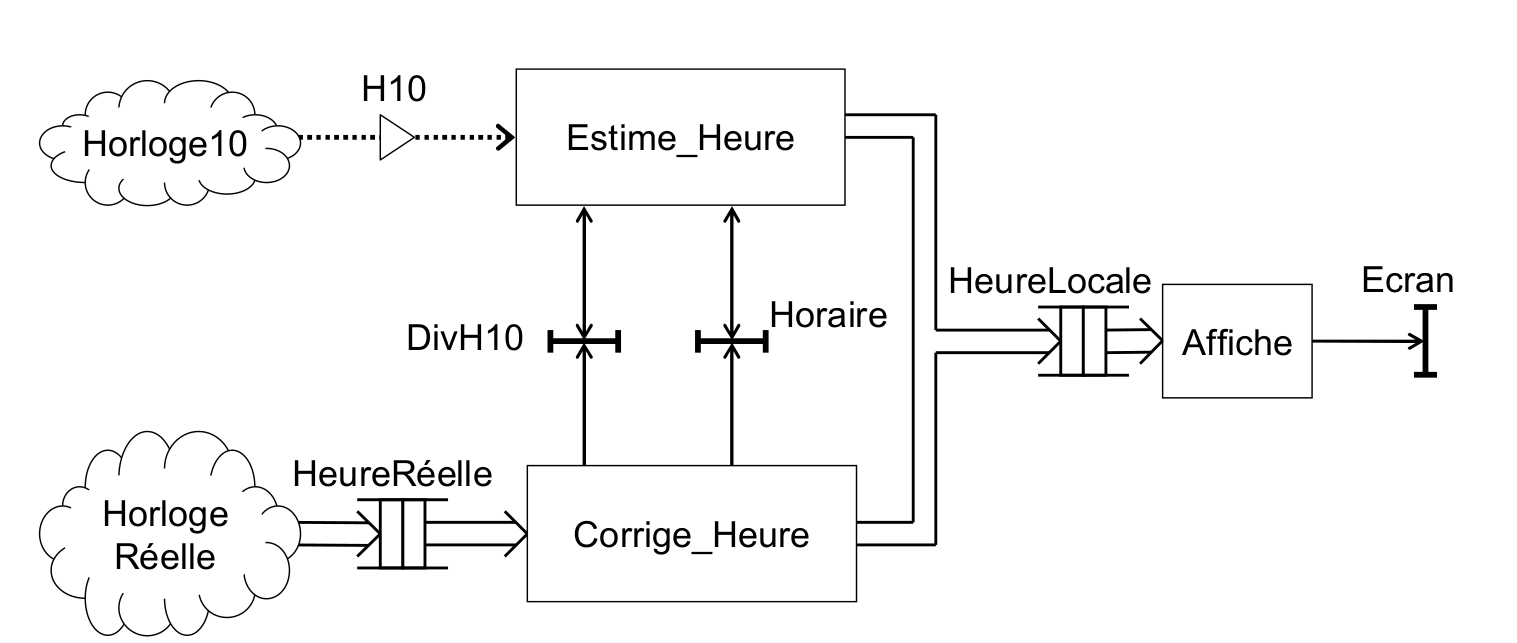
\includegraphics[width=13cm]{photo/situation}
		\caption{Sortie sur la console}
		\label{fig:structure_fontionnelle}
	\end{figure}
	
	L’application consiste à afficher sur Ecran, l’heure (heure, minute, seconde). L’heure
peut être obtenue par estimation à partir d’une horloge à 10Hz (H10) et pour éviter les
dérives, l’heure réelle est reçue par l’intermédiaire de HeureRéelle (heure, minute, seconde).
	Pour information, afin de limiter la longueur des observations, la base de temps de
l’environnement est beaucoup plus rapide que la seconde.
	

	\subsection*{Fonction Estime\_Heure}
	
	
	Action activée sur H10, événement périodique apparaissant 10 fois par seconde. Elle
incrémente la variable DivH10 si elle est inférieure à 9, sinon elle met la variable à 0 et la
variable Horaire est incrémentée d’une seconde. Un message est transmis dans HeureLocale.
	Le message indique que la valeur transmise est une valeur estimée et contient la nouvelle	valeur de Horaire.
	
	\subsection*{Fonction Corrige\_Heure}
	
	Action activée sur HeureRéelle. Elle copie la valeur reçue dans Horaire, met la
variable DivH10 à 0 et transmet un message dans HeureLocale. Le message indique que la
valeur transmise est une valeur réelle et contient la nouvelle valeur de Horaire.
	
	\subsection*{Fonction Affiche}
	
	Cette fonction copie sur Ecran l’heure reçue par l’intermédiaire de HeureLocale en
indiquant s’il s’agit de l’heure estimée ou de l’heure réelle (c’est la seule tâche ou vous
pouvez faire un printf).\\
	
	
	Le réseau de Pétri qui décrit le comportement des fonctions \texttt{Estime\_Heure} et \texttt{Corrige\_Heure} est donné à la figure \ref{fig:reseau_petri} ci-dessous.
	
	
	\begin{figure}[H]
		\centering
		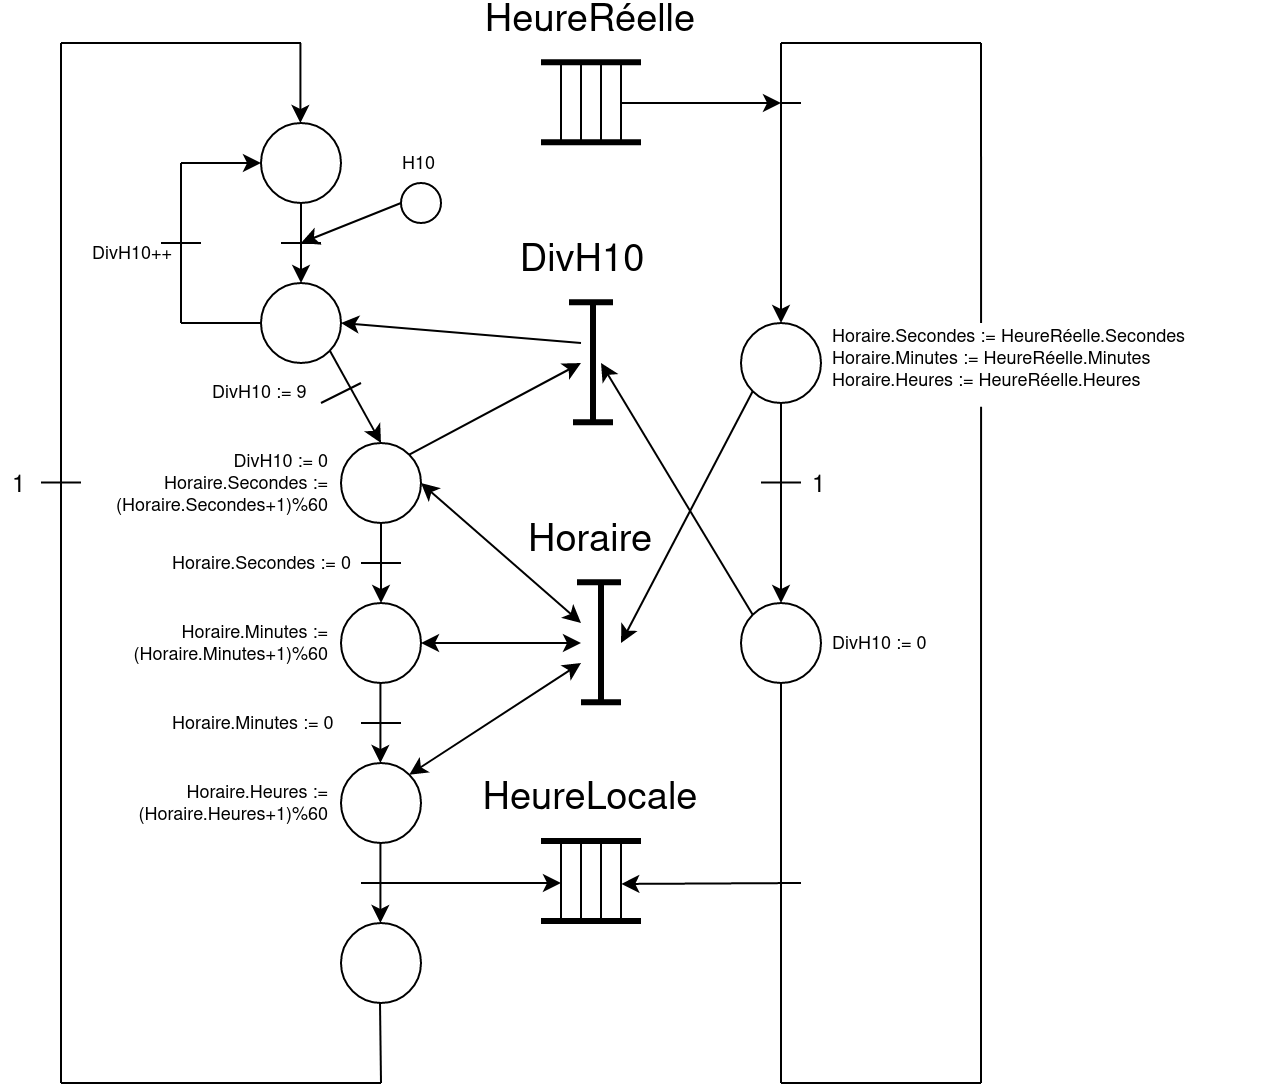
\includegraphics[width=13cm]{photo/reseau_petri}
		\caption{Sortie sur la console}
		\label{fig:reseau_petri}
	\end{figure}
	
	Dans ce réseau on est en présence de deux variables partagées \texttt{Div10} et \texttt{Horaire}. Une question logique à ce poser est : doit on mettre des sémaphores pour éviter des exclusions mutuelles ?\\
	
	La réponse est non car l'environnement est synchrone. Les tâches \texttt{Estime\_Heure} et \texttt{Corrige\_Heure} sont prêtes en même temps puis s'activent en même temps. Cela implique une gestion simple des priorités. C'est pourquoi il est possible d'éviter la mise en place de sémaphore.\\
	
	
	
	\section{Solution classique}
	% Parler de la solution d'implémentation (prépa)
	
	Cette partie vise à mettre en place la solution décrite précédemment. Pour l'implantation sur VxWorks, il est nécessaire d'utiliser les éléments suivants :
	\begin{itemize}
		\item une tâche \texttt{Estime\_Heure};
		\item une tâche \texttt{Estime\_Heure};
		\item une tâche \texttt{Estime\_Heure};
		\item un sémaphore \texttt{H10};
		\item une file de message \texttt{FMHeureLocale};
		\item une file de message \texttt{FMHeureReelle};
		\item une variable partagé \texttt{DivH10};
		\item une variable partagé \texttt{horaire}.		
	\end{itemize}
	
	On précise que la variable \texttt{horaire} est d'un type prédéfini \texttt{type\_heure} qui contient les secondes, les minutes et les heures dans une structure.\\
	
	Pour le bon fonctionnement du programme, il est nécessaire d'attribuer des priorités aux différentes tâches.Dans l’environnement	VxWorks, la tâche de priorité la plus élevée est celle qui dispose du numéro de priorité le plus faible. La tâche de priorité 0 est la plus prioritaire et la tâche de fond est la tâche de priorité 255. On évite d’attribuer les priorités comprises entre 0 et 10, réservée à l’environnement VxWorks. Les priorités suivantes sont affectées aux tâches :
	
	\begin{table}[H]
		\centering
		\begin{tabular}{|c|c|}
			\hline
			Tâche & Priorité \\
			\hline
			\texttt{Estime\_Heure} & 13 \\
			\hline
			\texttt{Corrige\_Heure} & 14 \\
			\hline
			\texttt{Affiche} & 15 \\
			\hline
		\end{tabular}
		\caption{Attribution des priorités aux différentes tâches}
		\label{tab:priorite_taches}
	\end{table}
	
	\subsection{Validation du comportement}
	
	La figure \ref{fig:affichage_comportement_normal} montre la sortie de la console pour une exécution classique du programme.
	
	\begin{figure}[H]
		\centering
		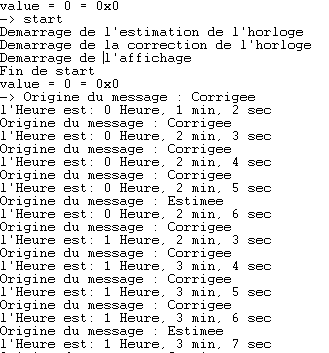
\includegraphics[width=8cm]{photo/affichage_normal/affichage_comportement_normal}
		\caption{Sortie sur la console}
		\label{fig:affichage_comportement_normal}
	\end{figure}
	
	Une fois l'initialisation des tâches effectués dans le \texttt{start}, nous observons un affichage de l'heure provenant des deux tâches. On note que l'heure affiché provient beaucoup plus souvent de \texttt{Corrige\_Heure} que de \texttt{Estime\_Heure}.
	
	
	\begin{figure}[H]
		\centering
		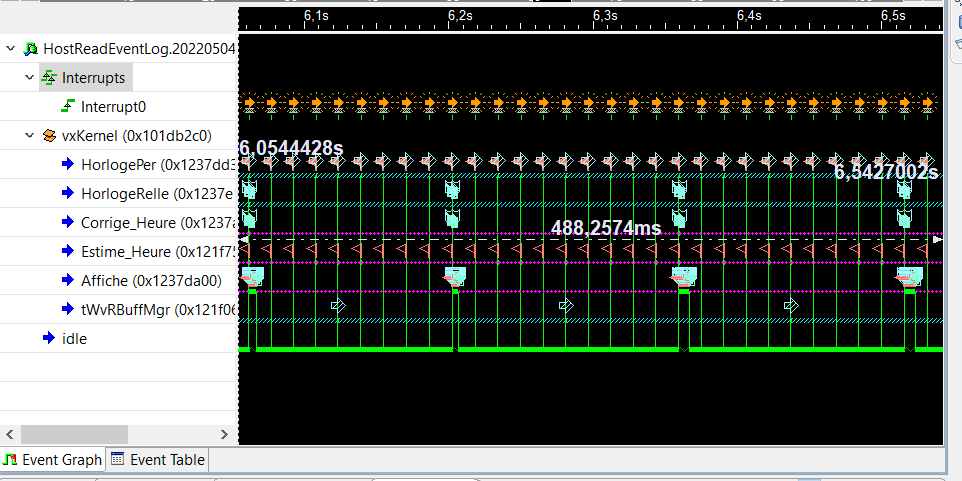
\includegraphics[width=16cm]{photo/affichage_normal/comportement_normal_fois_3}
		\caption{Sortie sur la console}
		\label{fig:affichage_comportement_normal}
	\end{figure}
	
	
	
	\begin{figure}[H]
		\centering
		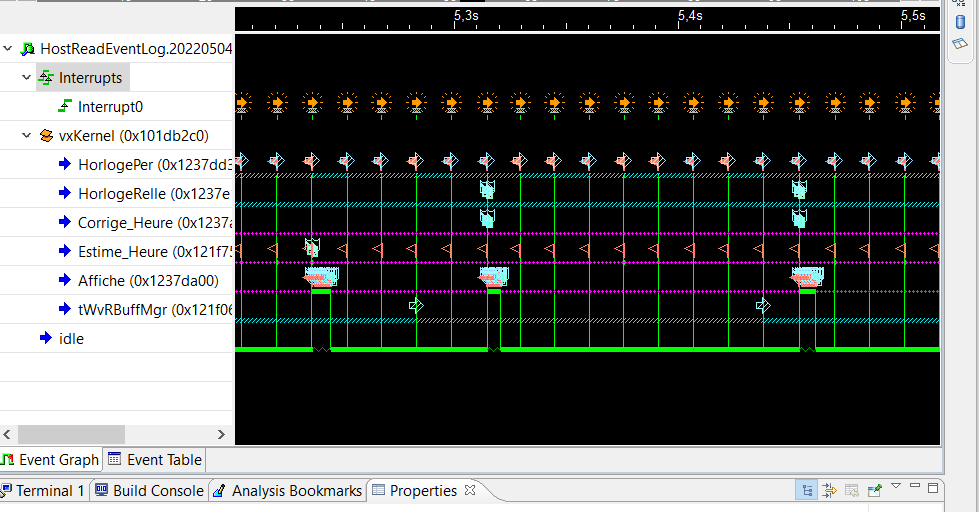
\includegraphics[width=16cm]{photo/affichage_normal/interruption_corrige_heure}
		\caption{Sortie sur la console}
		\label{fig:affichage_comportement_normal}
	\end{figure}
	
	Le code commenté de la solution à un utilisateur pour les priorités ci-dessus est disponible en Annexe 1. La simulation de la situation est lancée et analysée ci-dessous.


	\subsection{Asservissement de la boîte aux lettres}	
	
	La section qui suit s'intéresse au principe de l'asservissement de la boîte aux lettres. Il s'agit de comprendre le fonctionnement du système lorsque la file de message est pleine. Le cas de la file de message \texttt{HeureLocale} vide n'est pas considérée ici de part sa simplicité. En effet si celle-ci est vide alors la tâche \texttt{Affiche} appelle la fonction bloquante \texttt{msgQReceive} et attend l'émission d'un nouvel horaire. La suite abordera donc le cas de la file de message pleine. Afin d'assurer un remplissage complet de la file de message \texttt{HeureLocale}, le programme est modifié pour faciliter l'arrivée de cet événement. La taille de la file de message est réduite à 3 et une fonction de VxWorks nommée \texttt{taskDelay} est utilisée.\\
	Celle-ci prends en argument un entier correspondant au nombre de 'top' horloge du CPU virtuel à attendre avant de continuer la suite de la tâche \texttt{Affiche}. La durée d'exécution de la tâche \texttt{Affiche} est alors augmentée, ce qui laissera le temps à \texttt{Estime\_Heure} et \texttt{Corrige\_Heure} de remplir la file de message. Le choix est arbitraire et se porte sur 500 ms. Afin de déterminer le nombre de 'top' horloge à compter, la fonction \texttt{sysClkRateGet} est rentrée dans la console de VxWorks et renvoie la fréquence du CPU virtuel, ici 60 Hz. Le produit $60\times0.5$ donne 30 'top' horloge.\\
	La figure ci-dessous représente le diagramme d'activité global du système.
	
	
	\begin{figure}[H]
		\centering
		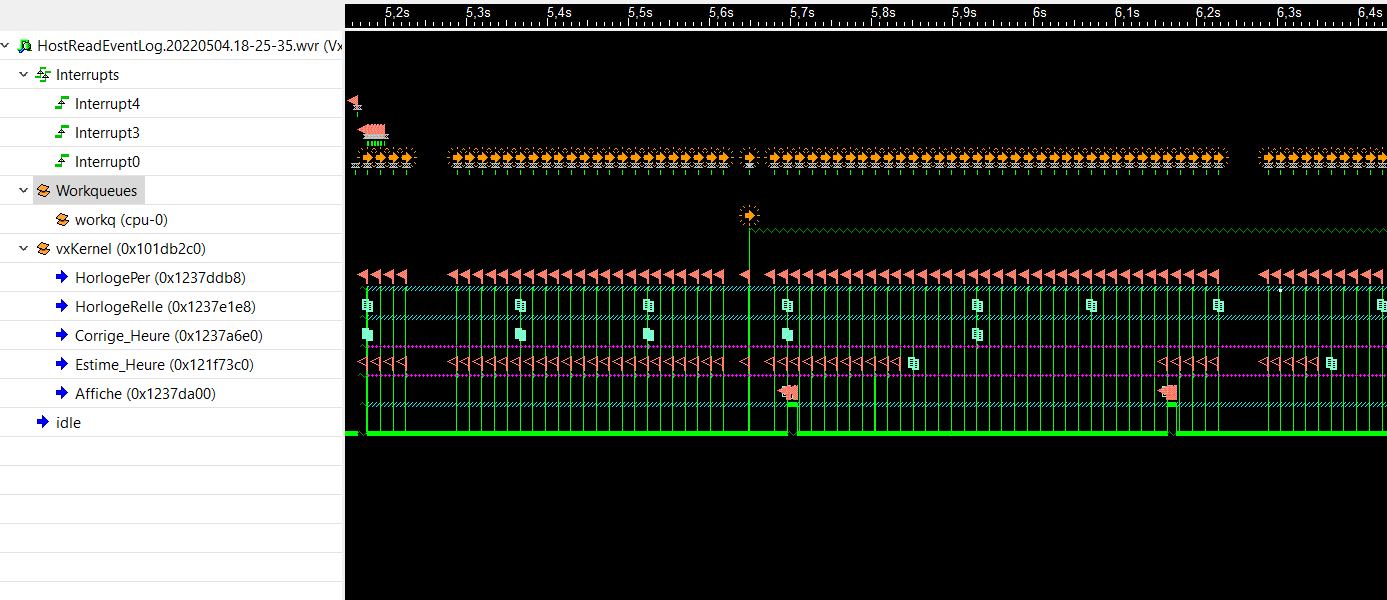
\includegraphics[width=1\linewidth]{../affichage_ralenti/vue_globale.PNG}
		\caption{Vue globale de la simulation}
		\label{fig:vue_globale}
	\end{figure}
	
	La simulation effectuée regroupe l'ensemble des tâches du système comme \texttt{Estime\_Heure},\\ \texttt{Corrige\_Heure} et \texttt{Affiche}. Celle-ci regroupe également le comportement temporel de l'environnement avec \texttt{HorlogePer} et \texttt{HorlogeRéelle} qui sont respectivement les entités \texttt{Horloge10} et \texttt{HorlogeRéelle}. Parmi cet ensemble d'éléments, les plus en haut sont les plus prioritaires et ceux qui sont les plus en bas sont les moins prioritaire.\footnote{Pour remarque, il est déconseillé d'attribuer une priorité supérieure à 100 pour une tâche de fond. En effet dans ce cas la tâche \texttt{RingManager} ne sera jamais exécutée ce qui peut provoquer le plantage de VxWorks.}\\
	Sur la ligne \texttt{Estime\_Heure}, la tâche récupère convenablement le sémaphore \texttt{H10} et arrive un moment où celui-ci n'est plus pris. Cet événement témoigne du remplissage complet de la file de message \texttt{HeureLocale}. Une analyse étape par étape démontre ce phénomène.
	
	\begin{figure}[H]
		\centering
		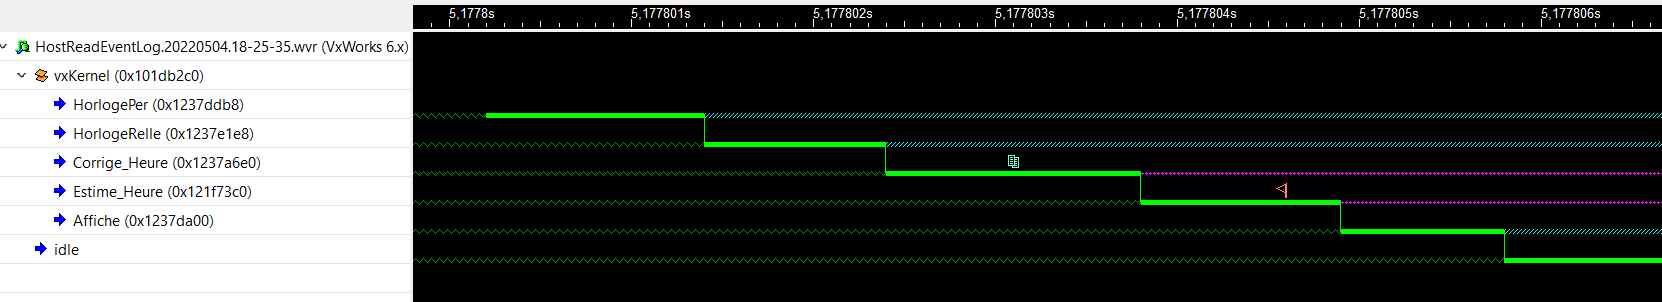
\includegraphics[width=1\linewidth]{../affichage_ralenti/lancement des taches.PNG}
		\caption{Initialisation des tâches}
		\label{fig:init_task_classique}
	\end{figure}

	La figure ci-dessus représente l'initialisation des tâches avant de rentrer dans les boucles infinies. Dans le cas de \texttt{Corrige\_Heure}, celle-ci s'initialise et rentre dans la boucle infinie, puis appelle la fonction \texttt{msgQReceive} et reste bloquée dans l'attente d'une donnée dans la file de message \texttt{HeureRéelle}.\\
	En ce qui concerne \texttt{Estime\_Heure}, cette tâche s'initialise et rentre dans la boucle infinie pour au final être bloquée car aucun sémaphore \texttt{H10} a été émis. Par la suite, la figure suivante représente le premier envoi d'une donnée dans la file de message \texttt{HeureRéelle}. L'appel de la fonction \texttt{msgQSend} est effectué de la part de \texttt{HorlogeRéelle}. Le noyau temps-réel donne la main à \texttt{Corrige\_Heure} qui appelle \texttt{msgQSend}, en effet à l'initialisation celle-ci est restée bloquée avec \texttt{msgQReceive}, l'envoi d'une donnée dans la file de message a permis à cette tâche d'être de nouveau prête. La donnée est donc envoyée dans la file de message \texttt{HeureLocale} et \texttt{Corrige\_Heure} reboucle et revient à nouveau dans l'attente d'une donnée, ici remarquable par l'appel de la fonction \texttt{msgQReceive}. La tâche \texttt{Affiche} n'est pas présente, ce qui dans une utilisation normale devrait être le cas. En regardant les temps, l'initialisation de \texttt{Affiche} se termine à 5,177 ms environ. L'envoi d'un premier message est effectué vers 5,178 ms. Seulement une microseconde sépare ces deux événements, la tâche \texttt{Affiche} est bloquée par la fonction \texttt{taskDelay} pendant une demie-seconde, avant l'appel de la fonction \texttt{msgQReceive}. Le message sera donc récupéré seulement vers 5,7 ms.
	
	\begin{figure}[H]
		\centering
		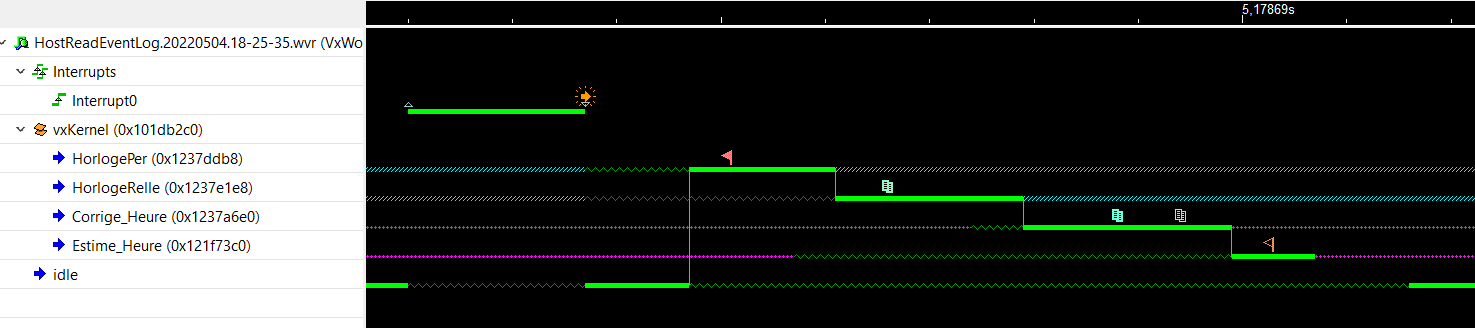
\includegraphics[width=1\linewidth]{../affichage_ralenti/1er_envoi_HeureReelle.PNG}
		\caption{Premier envoi d'une donnée dans la file de message \texttt{HeureRéelle}}
		\label{fig:premier_envoie_heurereelle}
	\end{figure}

	Il est possible de remarquer qu'entre temps, \texttt{HorlogePer} a émis le sémaphore \texttt{H10} qui a ensuite été récupéré par \texttt{Estime\_Heure}. Aucun appel de \texttt{msgQSend} est effectué, il est donc possible de déduire que la variable partagée \texttt{DivH10} est inférieure à 10. Ce même comportement est visible de nombreuses fois, la figure suivante le précise.
	
	\begin{figure}[H]
		\centering
		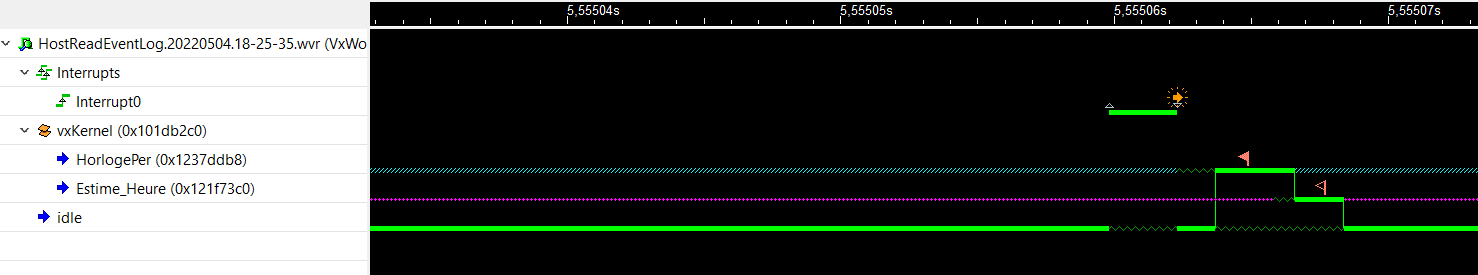
\includegraphics[width=1\linewidth]{../affichage_ralenti/estime_heure_h10_incremente.PNG}
		\caption{Émission du sémaphore \texttt{H10} et prise de celui-ci par \texttt{Estime\_Heure} dans le cas où la variable partagée \texttt{DivH10} est inférieure à 10}
		\label{fig:estime_heure_h10_incremente}
	\end{figure}

	D'après la figure (\ref{fig:vue_globale}), entre l'initialisation et jusqu'à 5,6 ms environ, 3 \texttt{msgQSend} sont effectués de la part de \texttt{HorlogeRéelle}. Ces 3 messages sont récupérés par \texttt{Corrige\_Heure} et envoyés dans la file de message \texttt{HeureLocale}. Celle-ci est alors pleine.\\
	La figure suivante représente le moment où \texttt{Affiche} sort de la fonction bloquante \texttt{taskDelay}. Avant cela un message est envoyé dans la file de message \texttt{HeureRéelle}, la tâche \texttt{Corrige\_Heure} sort de la fonction bloquante et appelle ensuite la fonction \texttt{msgQSend} à 5,696205 ms. Cet appel ne signifie pas que le message est envoyé dans la file de message, en l'occurrence la tâche \texttt{Corrige\_Heure} reste bloquée car la file de message \texttt{HeureLocale} est pleine. 

	\begin{figure}[H]
		\centering
		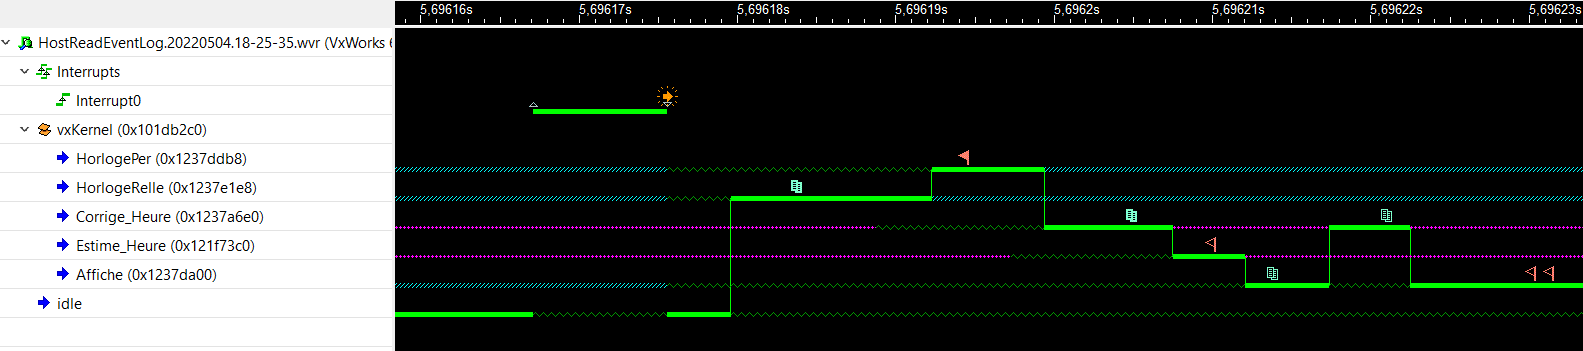
\includegraphics[width=1\linewidth]{../affichage_ralenti/premire_fois_affiche_recois.PNG}
		\caption{Réception et affichage du premier message contenu dans \texttt{HeureLocale}}
		\label{fig:premiere_fois_affiche_recois}
	\end{figure}

	À environ 5,696215 ms, la tâche \texttt{Affiche} est libérée de la fonction \texttt{taskDelay} et récupère le premier message. La file de message passe à 2 éléments. Mais celle-ci repasse immédiatement à 3 messages. En effet comme expliqué ci-dessus, la tâche \texttt{Corrige\_Heure} est bloquée dans la fonction \texttt{msgQSend} dans l'attente d'une place dans la file de message. Pour preuve, la suite du diagramme montre que \texttt{Corrige\_Heure} appelle la fonction \texttt{msgQReceive}. En ce qui concerne \texttt{Affiche}, celle-ci redevient bloquante à cause de l'appel de \texttt{taskDelay}, et ceci pour encore 500 ms.\\
	
	La file de message \texttt{HeureLocale} est à ce moment là composée de 3 messages, celle-ci est donc remplie. La figure ci-dessous montre lorsque la variable partagée \texttt{DivH10} vaut au moins 10, ce qui n'a jamais été le cas si l'on compte sur la figure (\ref{fig:vue_globale}) l'ensemble des \texttt{semGive} de \texttt{HorlogePer}. À ce moment là \texttt{Estime\_Heure} est enfin amenée à envoyer un message dans \texttt{HeureLocale}. Cela est tenté par l'appel de la fonction \texttt{msgQSend} contenue dans \texttt{Estime\_Heure}. Cependant la file de message \texttt{HeureLocale} est pleine. La tâche \texttt{Estime\_Heure} est alors bloquée par \texttt{msgQSend}. 
	
	\begin{figure}[H]
		\centering
		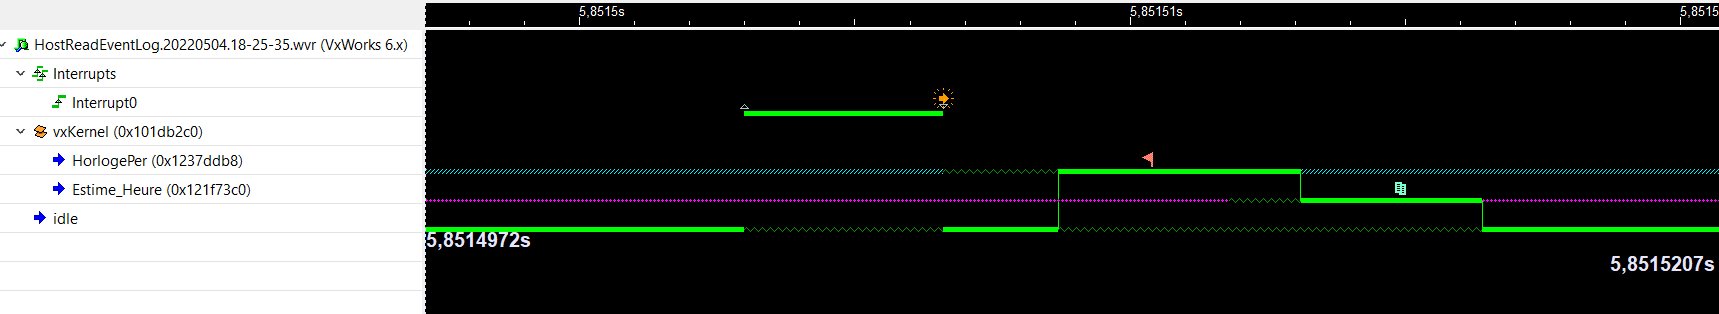
\includegraphics[width=1\linewidth]{../affichage_ralenti/premiere_fois_EstimeHeure_envoi.PNG}
		\caption{Première tentative d'envoi d'un message dans \texttt{HeureLocale} par \texttt{Estime\_Heure}}
		\label{fig:premiere_fois_estime_heure_envoie}
	\end{figure}

	Cela permet d'expliquer pourquoi sur la figure (\ref{fig:vue_globale}) il n'y a une absence de drapeaux \texttt{semTake} de la part de \texttt{Estime\_Heure}. En effet, celle-ci est bloquée par \texttt{msgQSend}, et ceci jusqu'à ce que \texttt{Affiche} soit libérée du \texttt{taskDelay}. Également sur la figure (\ref{fig:vue_globale}) il est possible de remarquer qu'un message est envoyé dans \texttt{HeureRéelle}. Celui-ci est récupéré et \texttt{Corrige\_Heure} tente de l'envoyer mais \texttt{HeureLocale} est pleine. Ce qui montre qu'ensuite tous les messages placé dans \texttt{HeureRéelle} en pourront pas être récupéré par \texttt{Corrige\_Heure} car cette tâche est également bloquée par \texttt{msgQSend}.\\
	
	Pour conclure sur cette section, il a été vu le comportement du système lorsque la file de message \texttt{HeureLocale} est pleine. Les contraintes temps-réel sont nullement respectées lorsque la tâche \texttt{Affiche} est moins cadencée que ces compères \texttt{Estime\_Heure} et \texttt{Corrige\_Heure}. Il est alors impératif d'avoir une tâche \texttt{Affiche} très réactive afin de vider le plus rapidement possible la boîte aux lettres.

	\subsection{Différences liées au type de sémaphore}
	
	\section{Variante}
	
	Le système conçu est capable d'estimer l'heure à l'aide du bloc \texttt{Estime\_Heure}. Cela est réalisable à l'aide du sémaphore \texttt{H10}, envoyé par l'entité \texttt{Horloge10}. Dans le cas où, pour quelconque raison, l'entité \texttt{Horloge10} n'effectue plus son rôle, la situation est critique et le système n'est plus capable d'estimer l'heure.

	\section{Conclusion}

	
\end{document}
